\section{System's Perspective}
%The report doesn't need to be structured in subsections to answer each question. The most important is that all these questions are answered in some way throughout the System's perspective section.

\subsection{Architecture and Design}

\subsubsection{Overview}
Below is a deployment diagram of the system:
\begin{figure}[h!]
    \centering
    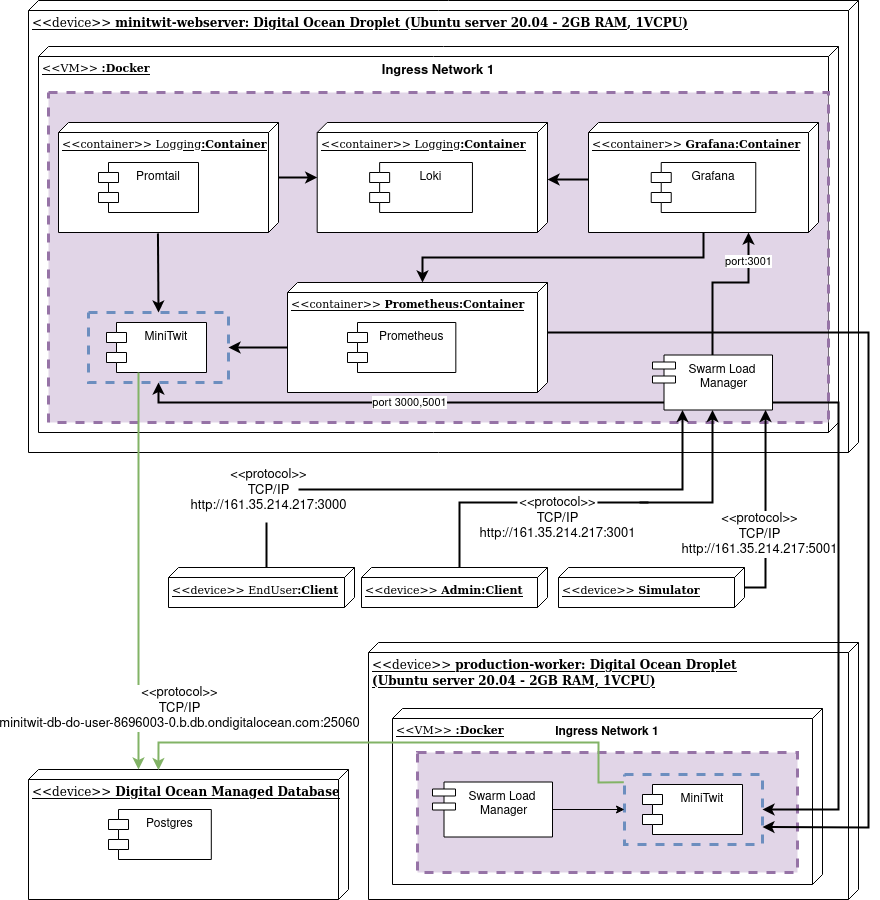
\includegraphics[width=1.2\linewidth]{report/images/system-architecture.png}
    \caption{System Architecture}
    \label{fig:arcitechture-overview}
\end{figure}
\todo{figuren skal opdateres med den nyeste version fra draw.io!}
\todo{Vi skal lige få afklaret om vi bruger promtail eller ej!}

Green arrow: database connection\\

The MiniTwit application runs on two droplets on Digital Ocean. A managed database hosted by Digital Ocean is used to host a Postgres database. The \textit{production-worker} droplet is running Docker swarm mode and is a swarm manager \cite{docker-swarm}. The \textit{minitwit-webserver} droplet is a worker node within the swarm. The MiniTwit application itself is grouped into the Minitwit component. The swarm hosts the Minitwit component in four replicas. The swarm also hosts the monitoring and logging stack in one replica. The monitoring and logging stack consists of Promtail to perform log aggregation, Loki to store and enable log query, Prometheus to collect and perform metric querying and finally Grafana to display the monitored and logged data. The swarm is run with a docker-compose.yml, which can be seen in appendix \ref{appendix:docker-compose}. \\
Furthermore, the swarm uses Dockerhub to pull all images for the services.
\\
Below is a decomposition of the Minitwit component:

\begin{figure}[h!]
    \centering
    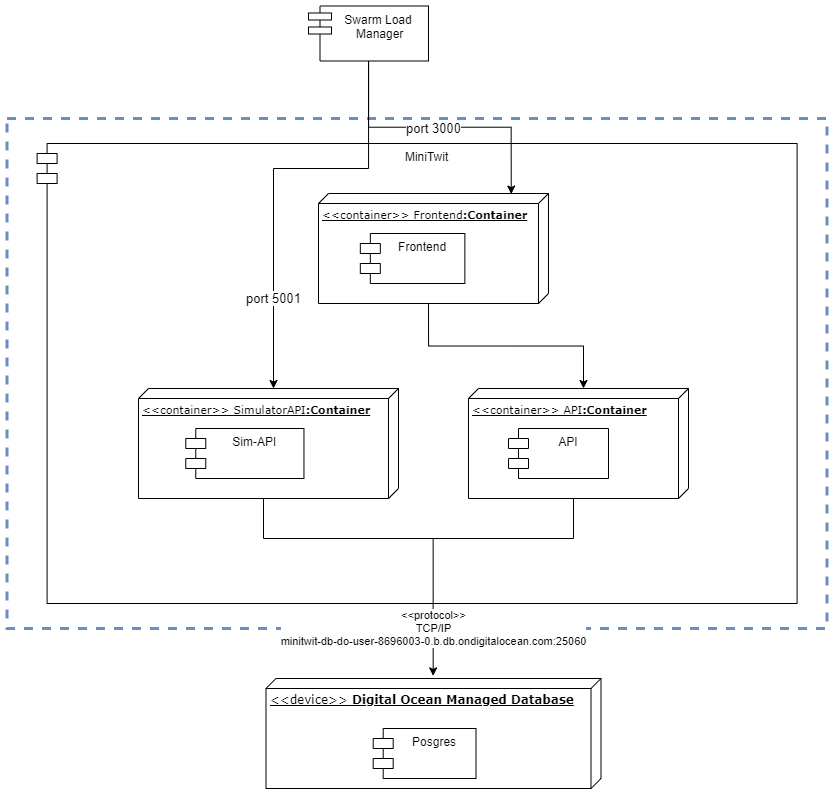
\includegraphics[width=1.1\linewidth]{report/images/minitwit-decomposition.png}
    \caption{MiniTwit Component Decomposition}
    \label{fig:arcitechture-overview}
\end{figure}

The Minitwit component is an abstraction to increase readability in the UML drawing and is therefore not a single container hosted in the swarm. The component consists of the front-end, API for the simulator (Sim-Api) and the API for the front-end. The simulator uses the \textit{Sim-API} service and the \textit{Frontend} uses the \textit{API} service.

\subsubsection{Design choices}

%TA used 3+1 view model. 
%Deployment diagram should be enough. 
%Maybe add package diagram - of how the api works with the different components.


The \textit{Frontend} service is written in React.js. Both the \textit{Sim-API} and \textit{API} are API's running on Node.js and exposes a RESTful API implemented with Express.js. \\
The rationale behind using javascript for both the front-end and back-end was that all of the team members were experienced with javascript. It is also a light-weight solution compared to a C\# implementation which is much more complex in terms of sub modules and interfaces. Also, developing with javascript is quick as each change in the source code is re-compiled in run-time during development, making debugging very easy.\\
\\
Below is a component diagram of the back-end illustrating the simplicity:

\begin{figure}[h!]
    \centering
    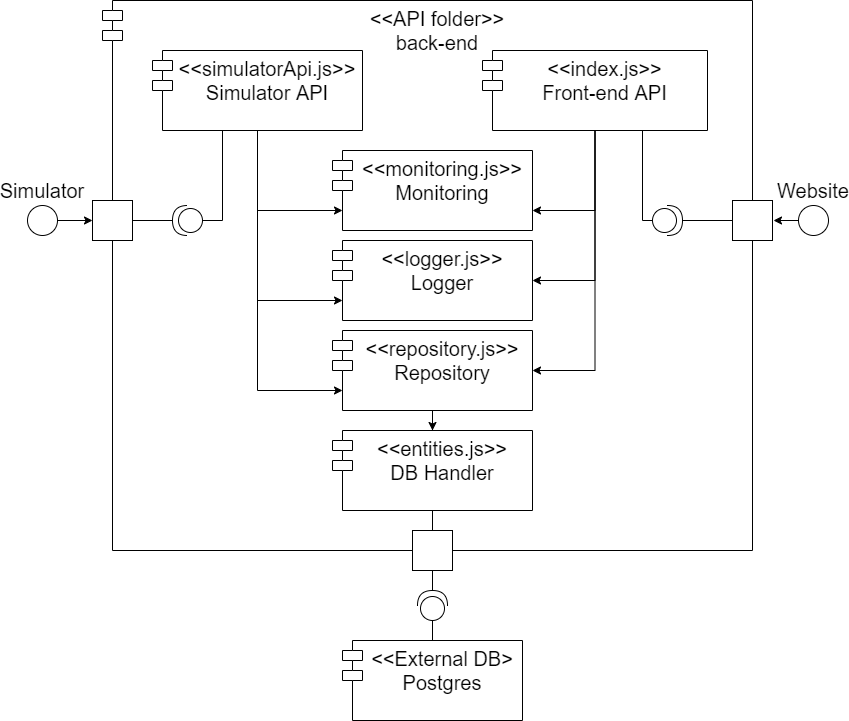
\includegraphics[width=1\linewidth]{report/images/component-diagram.png}
    \caption{Back-end Component diagram}
    \label{fig:back-end-component-diagram}
\end{figure}

Each component in the back-end is one single file and there are no formal interfaces. Both APIs implements the endpoints and uses the rest of the components as helpers to resolve each request.\\
The following list breifly describes each component:
\begin{enumerate}
    \item Monitoring: Provides functionality to use metrics used for Prometheus
    \item Logger: Provides logger objects to perform logging
    \item Repository: Provides an object to query the database
    \item DB Handler: Provides a database object with the database connection and schema.
\end{enumerate}

A Postgres database was chosen as all of the team members had previous experience using it and because it is a relational database, which fits the purpose of this project. The Sequelize library is used in the \textit{DB Handler} as the database abstraction layer and was chosen because it is well documented \cite{sequelize} and has a large community on stackoverflow.

\newpage
\subsection{Dependencies}

\subsubsection{Front-end and back-end low level diagrams}
The following is a description of the UML syntax used in the next two UML diagrams:
\begin{enumerate}
    \item Squares: files that the team developed
    \item Circles: external libraries
    \item Arrow: build-/compile-time dependency
    \item Dashed arrow: run-time dependency
\end{enumerate}

The front-end has the following dependencies:
\begin{figure}[H]
    \centering
    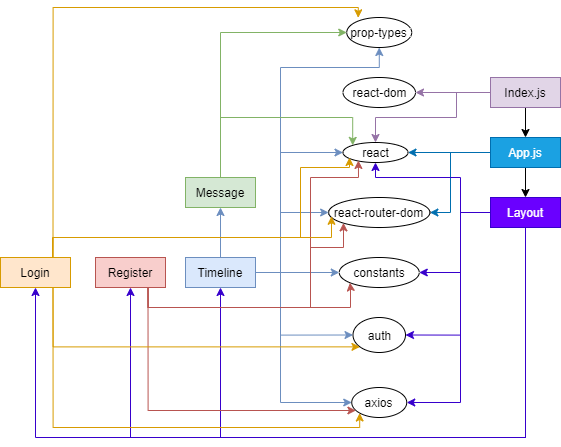
\includegraphics[width=0.9\linewidth]{report/images/Frontend-dependencies.png}
    \caption{Front-end dependency diagram}
    \label{fig:front-end-depencency-diagram}
\end{figure}
The squares are here components. Colors have here been used to improve the readability by each component having their own color. \\
The source code for this diagram is located at the Minitwit/Frontend folder.

\newpage
The back-end has the following dependencies:
\begin{figure}[H]
    \centering
    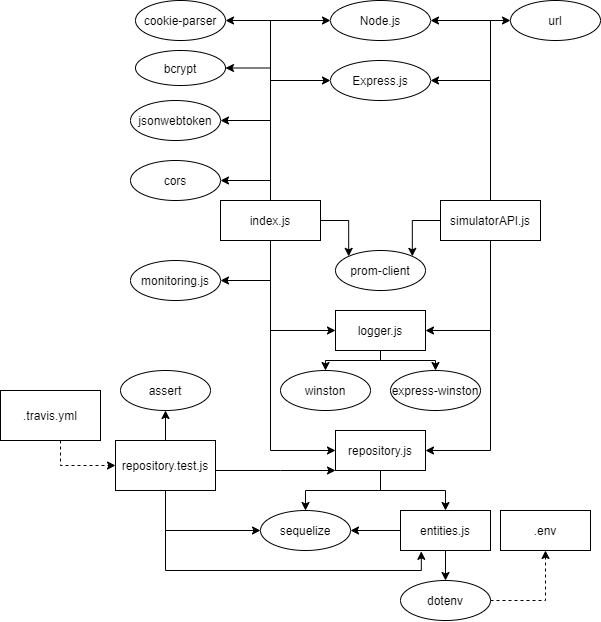
\includegraphics[width=1\linewidth]{report/images/backend-dependencies.png}
    \caption{Back-end dependency diagram}
    \label{fig:back-end-depencency-diagram}
\end{figure}

The source code for this diagram is located at the Minitwit/API folder.
All dependencies in the front-end and back-end uses the last release of the current major release. E.g. the \textit{bcrypt} dependency is \string^5.0.0 and will use future releases up until before the next major release: v6.0.0.

\subsubsection{The big picture}


\begin{figure}[H]
    \centering
    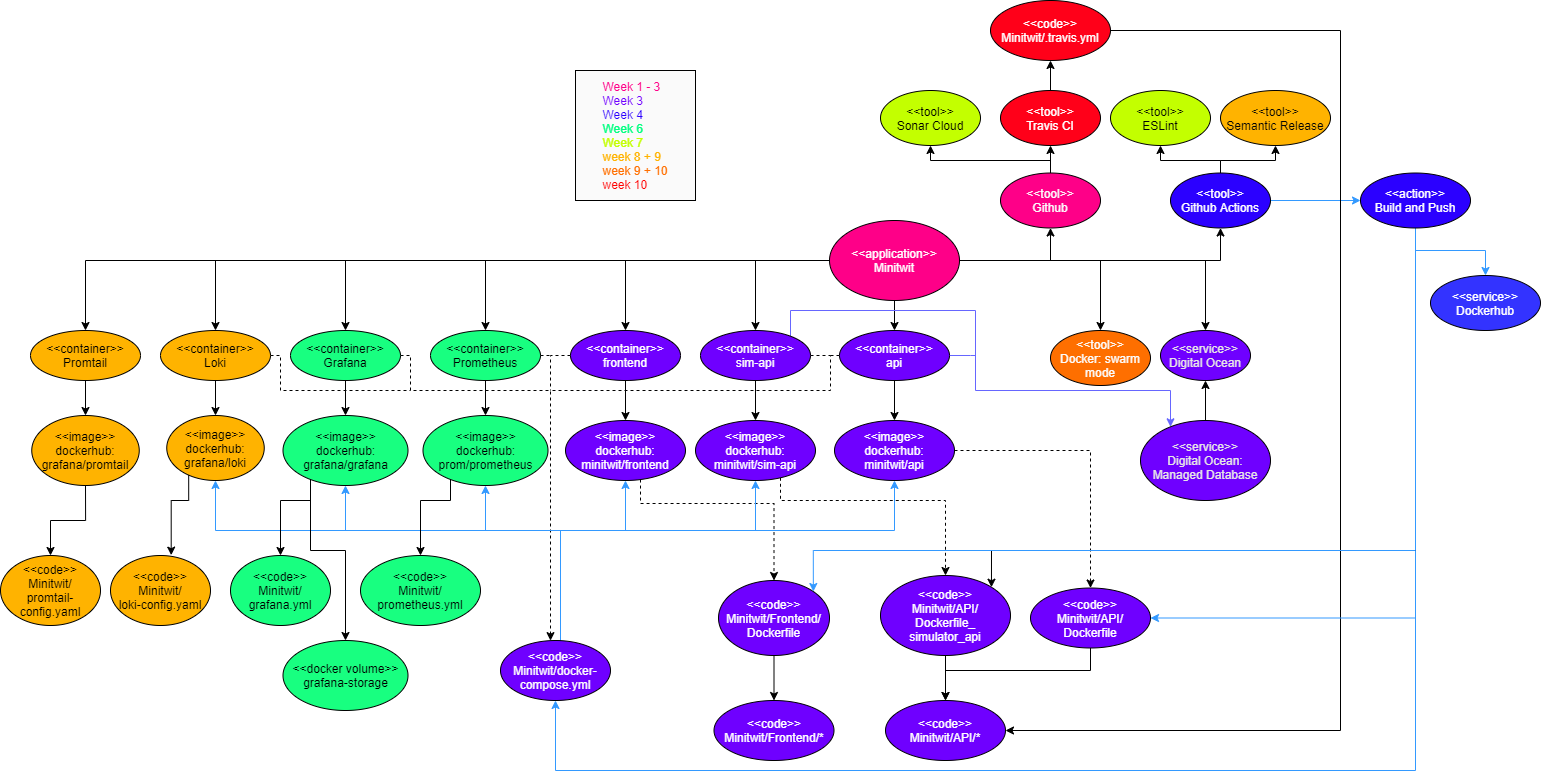
\includegraphics[scale=0.25, left]{report/images/system-dependencies.png}
    \caption{System dependencies. \href{https://github.com/Niels-Frederik/MiniTwit/blob/main/report/images/system-dependencies.png}{Click here for full size image}}
    \label{fig:system-depencencies}
\end{figure}

The following describes the UML syntax:
\begin{enumerate}
    \item Full line arrow: dependency
    \item Stippled line arrow: retired dependency
    \item Colored line arrow: for readability purpose only
\end{enumerate}
The diagram displays the dependencies of the project at a high level of abstraction. The various dependencies are color-coded such that the color corresponds to the week the dependency was introduced. 
\\
The dependencies of the front-end and back-end are omitted as they are described in figure \ref{fig:front-end-depencency-diagram} and \ref{fig:back-end-depencency-diagram}.

\subsection{Describe the current state of your systems, for example using results of static analysis and quality assessment systems.}
\todo{Skal laves}

\subsection{Describe briefly, if the license that you have chosen for your project is actually compatible with the licenses of all your direct dependencies.}
The ScanCode toolkit\cite{scancode} were used to scan for all licenses within the MiniTwit repository. The scan here outputted several permissive licenses where the most relevant were MIT and Apache-2.0. Furthermore, the most important finding was that no version of the GPL license were present. This is important, as the GPL is a copyleft license which would require MiniTwit to be a free open-source license\cite{gpl}. Hence, since no copyleft licenses such as GPL are in the project, MiniTwit has a variety of licenses to choose from.\\
The group chose the permissive MIT license in order to provide everyone with the free right to use the API, as well as keeping the developer team free from being liable of any claims made against any possible damage caused by the API.

\subsection{Service Level Agreement}
The SLA mentions that the API guarantees an uptime of 100\%\\
Vores SLA "https://github.com/Niels-Frederik/MiniTwit/blob/main/API/SLA.md"
TA's omtale vdr. SLA: "https://github.com/LazyOpsDev/Minitwit/blob/develop/report/report.md"
\todo{Læs i SLA'en hvordan uptime udregnes. Der skal skrives her hvordan dataen konkret ser ud (se TAøs rapport), jeg gik i stå fordi vi bare skriver "failure" under nogen af dem, og ikke om det er client eller server fejl. Tænker Yarl har lavet det?}
